\begingroup
\definecolor{proofink}{HTML}{17293C}
\definecolor{proofframe}{HTML}{C3CFD8}
\definecolor{proofbg}{HTML}{F3F6F8}
\definecolor{proofknown}{HTML}{196D60}
\definecolor{proofpartial}{HTML}{AD6229}
\definecolor{prooffixed}{HTML}{486E91}
\resizebox{\linewidth}{!}{%
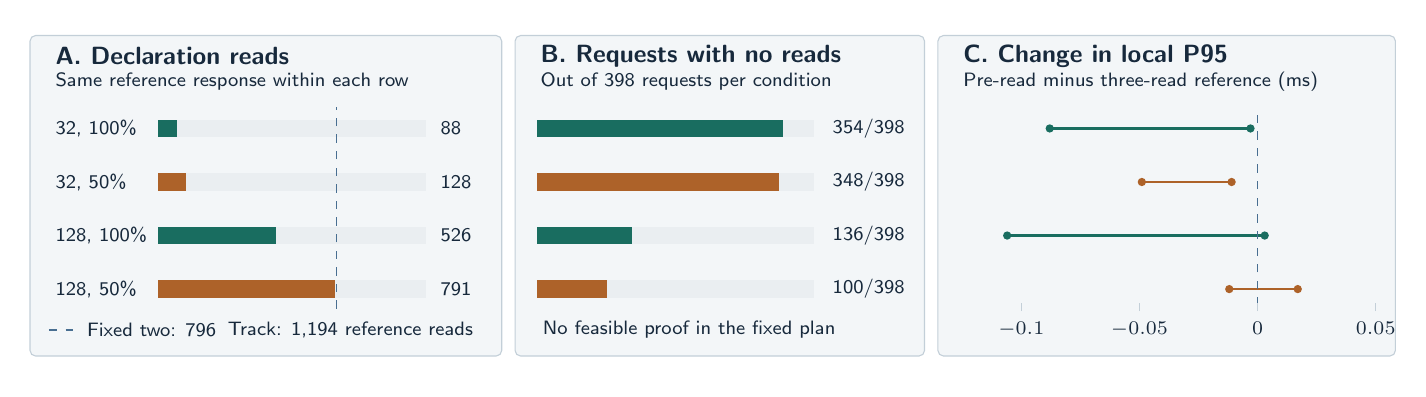
\begin{tikzpicture}[x=1cm,y=1cm,color=proofink,font=\sffamily\scriptsize,
  heading/.style={anchor=west,font=\sffamily\small\bfseries},
  panel/.style={rounded corners=2pt,draw=proofframe,fill=proofbg}]
  \path[use as bounding box] (0,0) rectangle (17.4,4.33);
  \draw[panel] (.03,.16) rectangle (6.02,4.23);
  \draw[panel] (6.19,.16) rectangle (11.39,4.23);
  \draw[panel] (11.56,.16) rectangle (17.37,4.23);
  \node[heading] at (.23,3.97) {A. Declaration reads};
  \node[heading] at (6.39,3.97) {B. Requests with no reads};
  \node[heading] at (11.76,3.97) {C. Change in local P95};
  \node[anchor=west] at (.23,3.65) {Same reference response within each row};
  \node[anchor=west] at (6.39,3.65) {Out of 398 requests per condition};
  \node[anchor=west] at (11.76,3.65) {Pre-read minus three-read reference (ms)};

  \foreach \desc/\vis/\y/\reads/\zero/\tone/\smallest/\largest in {
    {32}/100/3.05/88/354/proofknown/-.088/-.003,
    {32}/50/2.37/128/348/proofpartial/-.049/-.011,
    {128}/100/1.69/526/136/proofknown/-.106/.003,
    {128}/50/1.01/791/100/proofpartial/-.012/.017} {
    \node[anchor=west] at (.23,\y) {\desc{}, \vis\%};
    \fill[proofframe!35] (1.65,{\y-.11}) rectangle (5.06,{\y+.11});
    \fill[\tone] (1.65,{\y-.11}) rectangle ({1.65+.002856*\reads},{\y+.11});
    \node[anchor=west] at (5.12,\y) {\reads};

    \fill[proofframe!35] (6.47,{\y-.11}) rectangle (9.98,{\y+.11});
    \fill[\tone] (6.47,{\y-.11}) rectangle ({6.47+.00882*\zero},{\y+.11});
    \node[anchor=west] at (10.10,\y) {\zero/398};

    \draw[\tone,line width=.9pt] ({12.02+30*(\smallest+.12)},\y)
        -- ({12.02+30*(\largest+.12)},\y);
    \foreach \bound in {\smallest,\largest}
       \fill[\tone] ({12.02+30*(\bound+.12)},\y) circle (1.5pt);
  }
  \draw[prooffixed,dashed] ({1.65+796*.002856},.76) -- ({1.65+796*.002856},3.32);
  \draw[prooffixed,dashed] (.27,.49) -- (.57,.49);
  \node[anchor=west] at (.63,.49) {Fixed two: 796};
  \node[anchor=east] at (5.78,.49) {Track: 1,194 reference reads};

  \node[anchor=west] at (6.42,.49) {No feasible proof in the fixed plan};
  \draw[prooffixed,dashed] (15.62,.80) -- (15.62,3.32);
  \foreach \value in {-.10,-.05,0,.05} {
    \draw[proofframe] ({12.02+30*(\value+.12)},.73) -- ({12.02+30*(\value+.12)},.83);
    \node[anchor=north] at ({12.02+30*(\value+.12)},.71)
       {\pgfmathprintnumber[fixed,precision=2]{\value}};
  }
\end{tikzpicture}%
}
\endgroup
